\chapter{Impulsi lineari e impulsi logici}
Un \textbf{impulso lineare} \`e un impulso la cui informazione \`e contenuta nell'ampiezza e nella forma, un \textbf{impulso logico} \`e un impulso la cui informazione
\`e contenuta nel fatto che esso sia presente o meno e nell'istante in cui appare.\\
In genere una catena di acquisizione registra un impulso lineare, lo manipola e, ad un certo punto, lo trasforma in una serie di impulsi logici che vengono registrati.
\section{Classificazione degli impulsi lineari}
Gli impulsi lineari vengono classificati in:
\begin{itemize}
\item Impulsi veloci
\item Impulsi lenti
\item Impulsi dopo formatura
\end{itemize}
\subsection{Impulsi veloci}
Gli impulsi veloci sono segnali che vengono raccolti in circuiti con $\tau$ caratteristica molto piccola,
essi hanno quindi un \textit{rise time} e \textit{decay time} determinato dalle caratteristiche di raccolta della carica del rivelatore.
In genere questi impulsi hanno una \textbf{durata inferiore} a qualche $\mu$s e sono pi\`u \textbf{piccoli in ampiezza} (la polarit\`a viene determinata dall'alimentazione del rivelatore), per questo motivo soffrono di un \textbf{rapporto segnale-rumore peggiore}.\\
Gli impulsi veloci servono per trasformare informazioni temporali in quanto il fronte di salita ripido aumenta la risoluzione del dispositivo.
\subsection{Impulsi lenti}
All'opposto dei veloci, gli impulsi lenti sono segnali che vengono raccolti in circuiti con $\tau$ caratteristica grande. 
In genere il fronte di salita viene determinato dai tempi di raccolta della carica, mentre il fronte di discesa dalla $\tau$ caratteristica del circuito di raccolta,
per questo la $\tau$ viene scelta in modo da evitare il \textbf{deficit balistico}, ovvero lo smorzamento del segnale prima della raccolta completa della carica.
Per questo motivi vengono anche chiamati \textit{\textbf{tail pulses}} per via del fronte di discesa lungo.\\
Questi impulsi hanno un'ampiezza alta rispetto agli impulsi veloci e la loro polarit\`a e variabile, anche se spesso \`e negativa.
In conclusione, in questi segnali sono importanti l'ampiezza e il rise time (ovvero il tempo impiegato per passare dal 10\% al 90\% dell'ampiezza).
\subsection{Impulsi dopo formatura}
Sono impulsi lenti con tempi di decadimento nei microsecondi, in genere gli impulsi vengono formati per adattarli ai circuiti di lettura e analisi.
\section{Impulsi logici}
Esistono tre categorie:
\begin{itemize}
\item Impulsi logici standard (o TTL)
\item Impulsi logici NIM
\end{itemize}
\subsection{Impulsi TTL}
Sono impulsi a polarit\`a positiva, il livello 0 viene riconosciuto per tensioni tra -2V e 0V, mentre il livello 1 tra +4V e +12V.
La durata dell'impulso \`e nei $\mu$s e hanno una forma d'onda quadra.
\subsection{Impulsi veloci NIM}
Sono impulsi con tempi di salita nel ns (\`e necessario prendere cautele per effetti di riflessione), la loro polarit\`a \`e negativa e il segnale \`e in corrente.
L'ampiezza per il segnale 0 \`e tra -1mA e +1mA, per il segnale 0 \`e tra -14mA e -18mA.
\subsection{Impulsi di gate}
\textbf{NON sono impulsi logici}, serve a comandare e determinare il momento in cui un dispositivo \`e attivo e riceve segnale.
Ha la forma di un'onda quadra.
\section{Dispositivi per il trattamento degli impulsi}
\subsection{Linear-Linear}
\begin{itemize}
\item \textbf{Preamplificatore}, riceve in ingresso della carica e produce un impulso lineare a coda lunga 
\item \textbf{Amplificatore lineare}, riceve in ingresso un impulso lineare a coda lunga e produce un impulso formato ed amplificato
\item \textbf{Amplificatore a soglia}, riceve in ingresso un impulso formato e produce un segnale lineare proporzionale all'ampiezza del segnale in ingresso oltre la soglia.
\item \textbf{Allungatore di impulsi (\textit{Pulse stretcher}}, riceve un segnale lineare veloce in ingresso e produce un segnale formato della stessa ampiezza del segnale in input
%% elemento 5
\item \textit{Amplificatore sommatore}, riceve in ingresso pi\`u impulsi lineari formati e produce un segnale pari alla somma dei segnali in ingresso
\item \textbf{Modulo dei ritardi}, riceve un segnale e produce lo stesso segnale dopo un certo lasso di tempo
\item \textbf{Gate lineare}, riceve un impulso formato ed un impulso di gate e produce un segnale identico al segnale lineare se esso \`e in coincidenza con il gate
\end{itemize}
\subsection{Linear-Logic}
\begin{itemize}
\item \textbf{Discriminatori integrali}, riceve un impulso formato e produce un impulso logico se esso supera un livello di discriminazione
\item \textbf{Discriminatori differenziali}, riceve un impulso formato e produce un segnale logico se esso \`e compreso in una certa finestra di accettanza
\end{itemize}
\subsection{Logic-Linear}
\begin{itemize}
\item \textbf{Time to amplitude converter}, riceve in ingresso 2 segnali logici e produce un segnale lineare proporzionale all'intervallo di tempo tra l'arrivo dei due segnali
\end{itemize}
\subsection{Logic-Logic}
\begin{itemize}
\item \textbf{Modulo di coincidenza}, riceve impulsi logici e produce un segnale logico se essi appaiono entro un certo $\tau$ detto \textbf{resolving time}
\item \textbf{Modulo di anticoincidenza}, riceve impulsi logici e produce un segnale logico se si presenta un impulso solo in uno degli ingressi entro un $\tau$
\item \textbf{Scaler}, produce un impulso logico ogni tot impulsi logici
\end{itemize}

\section{Preamplificatori}
Se un dispositivo produce una quantit\`a di carica piuttosto elevata (come ad esempio un rivelatore Geiger) la tensione prodotta tramite la capacit\`a del rivelatore
pu\`o essere sufficiente per ottenere un impulso misurabile.
Spesso, tuttavia, \`e necessario utilizzare un \textbf{preamplificatore} (PRE) per aumentare l'ampiezza dell'impulso.\\
Questi dispositivi vengono messi molto vicini fisicamente ai rivelatori, per ridurre la capacit\`a dei cavi (la tensione \`e inversamente proporzionale alla capacit\`a),
hanno una resistenza di uscita molto bassa (per avere un $\tau = RC$ piccolo e non integrare il segnale), mentre quella in ingresso \`e molto elevata (per raccogliere completamente la carica).
Il segnale prodotto dal PRE \`e un segnale a coda lunga, in modo da non essere vincolante per la catena elettronica a seguire, in particolare il fronte di salita ha
tempi caratteristici molto brevi, mentre quello di discesa ha tempi nell'ordine dei 50-100 $\mu s$.\\
\subsection{Configurazioni dei preamplificatori}
\begin{figure}[htbp]
\begin{center}
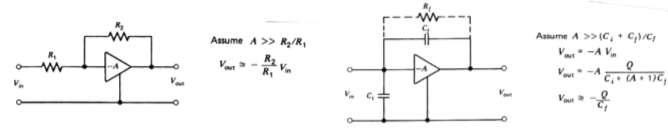
\includegraphics[scale=0.6]{./Immagini/ConfigurazioniPRE.png}
\caption{Configurazione voltage e charge sensitive}
\label{fig:configurazioniPRE}
\end{center}
\end{figure}
A sinistra nella figura~\ref{fig:configurazioniPRE} si vede la configurazione \textbf{voltage sensitive} del PRE:
se a monte del PRE \`e presente una capacit\`a costante il segnale in ingresso dal rivelatore sar\`a $Q/C$ per cui in uscita dal rivelatore,
se l'OP. AMP. ha un fattore di amplificazione sufficientemente grande, si ha un segnale pari a:
\begin{equation*}
V_{out} = - \frac{R_f}{R_i} V_{max} \propto Q
\end{equation*}
In molti rivelatori (come quelli a semiconduttore) la capacit\`a non \`e costante, per questo si opta per la configurazione \textbf{charge sensitive}:
Viene introdotta in parallelo a $R_f$ una capacit\`a di feedback, se l'amplificazione del OP. AMP. \`e sufficientemente grande allora:
\begin{equation*}
V_{out} = -A \frac{Q}{C_i + (A+1) C_f} \approx \frac{Q}{C_f}
\end{equation*}
In questo modo \`e possibile imporre una capacit\`a a piacere.
\subsection{Polarizzazione del rivelatore}
La tensione di polarizzazione del rivelatore pu\`o essere fornita attraverso la linea del preamplificatore.
Esistono due possibili configurazioni utilizzabili per fornire tale tensione, una accoppiata in AC e una accoppiata in DC.
\begin{figure}[htbp]
\begin{center}
	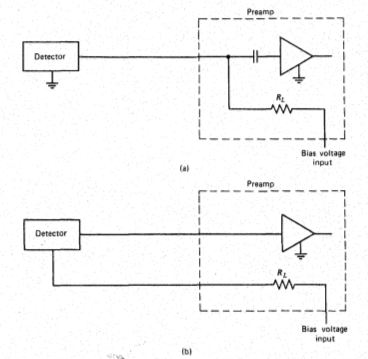
\includegraphics[scale=1]{./Immagini/TensPolarizzazione.png}
\caption{a) Accoppiamento in AC b) Accoppiamento in DC}
\label{fig:tensPolarizzazione}
\end{center}
\end{figure}
\subsubsection{Configurazione AC-coupled}
\`E la configurazione a) in figura~\ref{fig:tensPolarizzazione}, in questa configurazione la tensione di polarizzazione e la corrente di buio passano attraverso
la linea di resistenza $R_L$, il rivelatore \`e a massa.\\
Un condensatore di disaccoppiamento \`e posto all'ingresso del PRE in modo da poter scegliere $R_L$ senza modificare il segnale in uscita dal rivelatore.
La resistenza $R_L$ deve essere grande in modo da ridurre al minimo il rumore, tuttavia non pu\`o superare un certo valore in quanto attraverso di esse passa la corrente
di buio.
In presenza di correnti di buio troppo elevate si possono osservare cadute di tensione elevate lungo la linea, facendo cadere la tensione di polarizzazione applicata al rivelatore.
Per questo motivo la resistenza deve essere scelta in modo adeguato; in questi casi pu\`o essere utile regolare la tensione di polarizzazione fornita tenendo conto di questo fenomeno.
\subsubsection{Configurazione DC-coupled}
In questa configurazione la tensione di polarizzazione viene fornita direttamente al rivelatore che viene isolato dalla massa. 
Questa modalit\`a porta a rumori minori, tuttavia ha dei problemi legati al fatto che il segnale \`e accoppiato alla tensione di polarizzazione:
ci\`o implica che resistenze $R_L$ diverse possono portare a segnali diversi.
Dato che la corrente di buio passa dal PRE, in particolare dalla resistenza di feedback, correnti troppo elevate possono portare a segnali distorti per via delle tensioni
ai capi della resistenza. 
Un'alternativa \`e dato dall'uso di capacit\`a di feedback che integrano la corrente, poich\`e i segnali del PRE possono essere approssimati come dei gradini
questo significa che il fronte orizzontale diventer\`a crescente portando gradualmente alla saturazione del PRE.
I PRE possiedono sistemi di reset che, in presenza di una saturazione, riavviano il sistema, tuttavia essi introducono maggiori tempi morti.
Per questo in caso di correnti di buio molto intense possono portare a saturazioni pi\`u frequenti, per questo in tali casi l'accoppiamento in AC risulta una scelta obbligata.
\subsection{Preamplificatori nei vari rivelatori}
La catena elettronica di base in un preamplificatore \`e molto simile in tutti i rivelatori, con adattamenti a seconda delle caratteristiche del rivelatore.
Ad esempio i preamplificatori nei rivelatori a gas hanno correnti di buio minori, per questo \`e possibile introdurre resistenza $R_L$ molto elevate, per attenuare il rumore;
nei rivelatori a semiconduttore questo non pu\`o avvenire, in quanto le correnti sono maggiori.\\
Un'altra differenza pu\`o essere data dalla tensione di polarizzazione e dal suo isolamento, un rivelatore a gas richiede tensioni nell'ordine delle migliaia di volt,
mentre un semiconduttore nell'ordine delle centinaia, con la differenza che i cavi possono avere isolamenti differenti.\\
I segnali in uscita da un tubo fotomoltiplicatore di uno scintillatore sono piuttosto elevati, per questo i preamplificatori in questi rivelatori non hanno
caratteristiche troppo spinte, in quanto i problemi legati all'amplificazione ed al rumore sono ridotti. 
Per questo motivo i PRE hanno principalmente il ruolo di fissare il tempo caratteristico di un segnale.
Negli scintillatori \`e possibile lavorare anche con il segnale anodico, quindi in assenza di preamplificatore, in queste condizioni la forma del segnale
\`e fortemente dipendente dalla carattestiche fisiche dei cavi (come ad esempio la loro capacit\`a) e dell'elettronica a cascata e spesso la $\tau$ indotta da queste carattestiche pu\`o non essere ottimale.
I PRE generalmente non forniscono la tensione di alimentazione dello scintillatore, mentre l'alta tensione agisce sul tubo fotomoltiplicatore.
\subsection{Limite sul tasso di conteggi per la saturazione}
Un PRE pu\`o saturare in seguito ad un impulso eccessivo oppure in seguito a rate troppo elevati per pile-up in quanto la coda dell'impulso \`e lunga.\\
Una soluzione pu\`o venire dal diminuire il tempo caratteristico di discesa del segnale, tuttavia questo aumenta il rumore, in quanto entrano in banda passante 
nuove basse frequenze.\\
Se il rivelatore \`e accoppiato in continua allora la tensione di saturazione \`e data dalle correnti che provengono dal rivelatore, in particolare
se nel rivelatore viene depositata un energia $E$ e l'energia media di ionizzazione vale $\epsilon$, la carica liberata risulta:
\begin{equation*}
Q = \frac{E\cdot e}{\epsilon}
\end{equation*}
La corrente di saturazione sar\`a data dal rapporto tra la tensione di saturazione e la resistenza di feedback e sar\`a collegata ad un tasso massimo di ionizzazioni
che \`e possibile produrre, che indichiamo con $r_m$:
\begin{equation*}
I_{sat} = \frac{V_{sat}}{R_f} = \frac{E \cdot e}{\epsilon} \cdot r_m
\end{equation*}
Da questa relazione \`e possibile calcolare $r_m$ a partire dalle caratteristiche del PRE, in particolare \`e di interesse il limite \textbf{energia-rate}, ovvero
la quantit\`a massima di energia che si pu\`o mediamente misurare senza saturare il dispositivo:
\begin{equation*}
E \cdot r_m = \frac{V_{sat} \, \epsilon}{e\, R_f}
\end{equation*}
Per un rivelatore HPGe (High Purity GErmanium) ($\epsilon = 2.96$ eV) con $V_m = 10$ V e $R_f = 1$ G$\Omega$ esso vale $1.85 \cdot 10^5$ MeV/s.
\section{Amplificatori lineari}
L'amplificatore ha il ruolo di effettuare l'amplificazione e la formatura del segnale.
Il PRE preleva la propria alimentazione dall'amplificatore, per questo pu\`o essere soggetto a ground loop, in tal caso pu\`o essere necessario alimentare il dispositivo separatamente.
Tipicamente l'amplificatore \`e in grado di produrre in uscita segnali lineari tra i 0 e i 10 V, se il segnale in ingresso \`e maggiore di 10 V l'amplificatore satura,
distorcendo il segnale.
Il fattore di amplificazione deve essere scelto tenendo conto di questo fenomeno.\\
Per quanto riguarda la formatura del segnale, esse deve essere scelta in base ai rate di conteggio, la risoluzione, il rapporto segnale-rumore, il deficit balistico
e il pile-up.\\
In genere in caso di alti rate \`e meglio avere impulsi bipolari di larghezza limitata, per ridurre il pile-up, in caso di bassi rate queste restrizioni non sono presenti
per cui \`e meglio avere impulsi unipolari lenti, in modo da massimizzare la risoluzione energetica.\\
A bassi rate gli effetti collegati a pile-up e spostamenti della linea di base sono ininfluenti, per questo \`e meglio avere segnali con tempi caratteristici lunghi,
per minimizzare il rumore serie, tuttavia tempi caratteristici troppo lunghi possono aumentare il rumore per via del rumore parallelo, per questo esiste un valore ottimale.\\
Ad alti rate si ha un generale peggioramento del rumore, per via di problemi di pile-up e spostamento della linea di base, per questo il minimo si sposta
a tempi caratteristici inferiori, in generale per tempi caratteristici molto bassi gli effetti di alto rate vengono abbattuti e il rumore ritorna simile a
quello a basso rate.\\
Per sistemi a bassa risoluzione, in presenza di bassi rate, qualunque formatura va bene, mentre in presenza di alti rate \`e preferibile una formatura con
doppia linea di ritardo.\\
Nel caso di sistemi ad alta risoluzione per bassi rate \`e preferibile una formatura gaussiana o triangolare, mentre per alti rate una bipolare (per gli scostamenti
della linea di base).\\
\`E importante evitare che l'amplificatore saturi, specie ad alti rate, in quanto il tempo di recupero diventa maggiore in caso di saturazione, per questo \`e
importante avere un circuito che attivamente ristabilisca la linea di base.\\
In conclusione un amplificatore deve:
\begin{itemize}
\item Amplificare il segnale
\item Formare il segnale in modo da ottimizzare la misura di interesse
\item Formare il segnale in modo da evitare pile-up e saturazioni
\item Ottimizzare il rapporto segnale-rumore
\item Fornire circuiti di reiezione del pile-up e ristabilire in modo attivo la linea di base
\end{itemize}
\begin{figure}[htbp]
\begin{center}
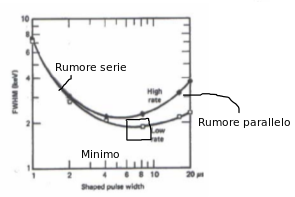
\includegraphics[scale=1]{./Immagini/RumoreSerieParallelo.png}
\caption{Rumore in funzione di rate e formatura}
\label{fig:RumoreSerieParallelo}
\end{center}
\end{figure}
\subsection{Amplificatori a soglia}
Sono dispositivi che amplificano la parte di impulsi sopra una determinata soglia, sono utili per analizzare particolari regioni dello spettro spalmandolo su tutto l'MCA.
Dato che esso registra la porzione di impulso sopra soglia, spesso questi segnali sono stretti, per questo \`e seguito da un pulse stretcher che dilata l'impulso
rendendolo analizzabile.
\section{Sistemi di conteggio}
\begin{figure}[htb]
\begin{center}
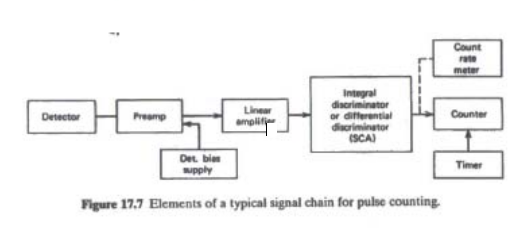
\includegraphics[scale=0.7]{./Immagini/CatenaConteggio.png}
\label{fig:catenaConteggio}
\end{center}
\end{figure}
Un sistema di conteggio deve misurare il rate di rivelazione.
\subsection{Discriminatori}
La presenza di un segnale in uscita dall'amplificatore viene verificata da un discriminatore a soglia.\\
Un discriminatore integrale produce un impulso logico se il segnale supera una determinata soglia, un discriminatore differenziale (o SCA, single channel analyzer) lo fa se il segnale entra
in una particolare finestra.
Spesso quest'ultimo \`e in grado di produrre segnali con un certo ritardo, scorrelando temporalmente il segnale.
\subsection{Contatori o scaler}
Lo scaler conta il numero di impulsi; esso pu\`o lavorare in due modalit\`a: in \textbf{preset time} il contatore conta il numero di impulsi in un determinato tempo
in base ad un clock interno o esterno, in \textbf{pulse count} esso fissa il numero di conteggi da raggiungere.\\
In questo dispositivo \`e fondamentale conoscere la risoluzione temporale o ''pulse pair resolving time`` per determinare l'intervallo di tempo
minimo tra due impulsi per essere conteggiati, in quanto essa determina il tasso massimo misurabile dal dispositivo.
\subsection{Tempo morto nei sistemi di conteggio}
\`E importante introdurre una correzione per il tempo morto del sistema, se esso \`e costante \`e possibile introdurla, mentre se esso varia, si fa in modo
di renderlo costante imponendolo come il pi\`u alto di tutta la catena.\\
Il tempo morto spesso non \`e determinato dal rivelatore (salvo contatori Geiger-Muller), ma dall'elettronica a cascata.
Il dispositivo con i tempi morti maggiori \`e il discriminatore, dove esso vale 1-2 $\mu$s pi\`u la durata dell'impulso.
\section{Analisi dell'ampiezza degli impulsi}
In generale rivelatori con FWHM media non necessitano di elettronica spinta, tuttavia per rivelatori ad alta risoluzione \`e necessario porre molta cura nella catena
di trattamento del segnale.\\
Il componente prioritario \`e dato dall'amplificatore, che, in caso di alte risoluzioni, deve utilizzare una formatura del segnale ottimale.
La strategia da usare deve essere in funzione del rate da analizzare, definiamo il \textbf{duty cicle}:
\begin{equation*}
D.C. = \Delta t \cdot r
\end{equation*}
con $r$ rate di impulsi.
Se il duty cicle \`e inferiore a $10^{-3}$ si pu\`o procedere con l'ottimizzazione della catena elettronica, se esso \`e maggiore di $10^{-1}$ \`e necessario
ridurre il rate in quanto si rischia di avere conflitti nell'elettronica.
\subsection{Deficit balistico}
Il deficit balistico consiste nel taglio dell'ampiezza del segnale per via della formatura.
In generale se la forma dell'impulso \`e costante allora la frazione tagliata \`e costante ed \`e possibile introdurre una correzione impulso per impulso,
altrimenti si assiste ad un peggioramento della risoluzione.\\
In alternativa risulta necessario allungare il tempo di salita dell'impulso, a scapito del rapporto segnale-rumore e del pile-up.
\section{Rumore}
Il rumore \`e una fluttuazione che si sovrappone al segnale in uscita dal dispositivo che degrada la FWHM, 
specialmente se esso si presenta nella regione iniziale della catena, dove il segnale \`e ancora piccolo.\\
Il rumore ha un proprio spettro che spazia dalle basse alle alte frequenze, in questo caso si parla di \textbf{rumore bianco}.
Posso distinguere il rumore bianco in \textbf{rumore serie} e \textbf{rumore parallelo}:
\begin{itemize}
\item il rumore serie \`e quello collegato a rumore termico nel FET o rumore Johnson (termico) nelle resistenze 
\item il rumore parallelo \`e legato a fluttuazioni della corrente di buio
\end{itemize}
Posso ridurre il rumore utilizzando filtri passa-alto e passa-basso che tagliano le frequenze in cui \`e presente unicamente il rumore.\\
Il rumore viene misurato in ENC (Equivalent Noise Charge): posto $v_{rms}$ la deviazione standard della distribuzione del rumore, ENC \`e il numero
di elettroni che, posto all'ingresso del PRE, produce una tensione pari a $v_{rms}$.
Dal ENC si ricava la FWHM attraverso la relazione:
\begin{equation*}
\text{FWHM} = \text{ENC} \cdot 2.35 \cdot \epsilon
\end{equation*}
\subsection{Microfonismo}
\`E un rumore dovuto a vibrazioni meccaniche nel dispositivo che modificano la capacit\`a, sono effetti piccoli che risultano visibili
solo in rivelatori con $C_{in}$ piccola. 
Il problema pu\`o essere risolto con filtri passa-basso, in quanto il rumore \`e a bassissima frequenza.
\subsection{Formatura e rumore}
Aumentando il tempo di formatura il rumore serie diminuisce, ma aumenta quello parallelo.
In aggiunta, esiste un terzo tipo di rumore, detto rumore 1/f, che non dipende dallo shaping time.
I tre rumori si combinano con una somma in quadratura:
\begin{equation*}
N^2 = N_S^2 + N_P^2+N_{1/f}^2
\end{equation*}
Esiste una formatura ottimale per cui i rumori serie e parallelo si compensano, tipicamente nei $\mu$s per i rivelatori a Si o Ge.\\
Dal punto di vista matematico, la cuspide infinita sembra avere il miglior rapporto segnale-rumore, tuttavia questa forma ha diversi problemi pratici:
ha il massimo a punta, il quale \`e difficilmente misurabile, ha una durata lunga, dando problemi di pile-up, ed \`e difficile da ottenere in pratica.
\section{L'impulso di gate}
L'impulso di gate comanda l'acquisizione del segnale, esso deve essere pi\`u lungo della durata del segnale e i dispositivi che utilizzano un gate devono attivarsi velocemente
quando esso si presenta.
\section{Tiratore di impulsi}
Produce impulsi di forma standard di ampiezza pari a quella in ingresso, viene utilizzato in presenza di impulsi veloci o stretti, per adattarli all'elettronica.